\chapter{Two fission modes in $^{178}$Pt}\label{chap:178Pt}

\section{Asymmetric fission in the region of $^{180}$Hg}
As mentioned in the introduction, fission is most well-studied in the region of the actinides (Z=90 to Z=103), as many naturally-occurring isotopes in this region are fissile. Within this region, there is a characteristic tendency for fission fragment yields to be asymmetric (that is, one light fragment and one heavy fragment), with the heavy peak centered around $A\approx140$. This has been understood as a manifestation of nuclear shell structure in the prefragments: doubly-magic $^{132}$Sn drives the nucleus towards scission, and once the neck nucleons are divided up between the two fragments, we end up with the heavy fragment A=140 peak. As one moves to the lower-Z actinides, however, this tendency becomes less and less pronounced as yields tend to become more symmetric. Below thorium, it was generally believed until recently (though mostly not tested) that yields would continue to be symmetric as there was no doubly-magic nucleus candidate that could drive the system toward asymmetry as there is with actinides.

However, it was reported in a 2010 study \cite{Andreyev2010} that neutron-deficient $^{180}$Tl undergoes beta-delayed fission, leading to intermediate state {\Hg} which then decays into two fragments of unequal mass. This finding triggered a flurry of theoretical papers hoping to describe this new and unexpected phenomenon (for instance, see \verb|\cite{some papers}|). A follow-up study using $^{178}$Tl \cite{Liberati2013} further established this as a region of asymmetric fission, and not just a one-time occurrence. Since then, other nuclei in the region have been studied, for instance using Coulex-induced fission reactions and compound nucleus (prompt?) fusion-fission reactions, and the finding is the same. 

Nuclei in this region have a number of unique features which make them interesting for study, even aside from the unexpected fragment asymmetry. Predicted fission barrier heights in this region are relatively-low (of the order of ~12 MeV), making them suitable for study using low-energy techniques such as $\beta$-delayed fission (maybe \cite{Andreyev2013} and the work at ISOLDE at CERN?) or Coulex-induced fission (maybe \cite{Martin2015} and the SOFIA (Studies On FIssion with Aladin) experiment/project/campaign). On the other hand, it has been found that compound nuclei formed in this region from particle-induced reactions tend to have high excitation energies, even for beam energies near the Coulomb barrier. This combination makes the region particularly well-suited for studies involving a variety of excitation energies.

Later experiments performed with isotopes in this region at different excitation energies have shown that, unlike the case of actinides where shell structure and fragment asymmetry is ``washed out'' at high excitation energies, mass asymmetric fragment distributions are a persistent feature of this mass region for various excitation energies. (A lot of good citations for this section can come from section 4.1.1 of \cite{Andreyev2018}) An up-to-date (as of around 2016) overview of nuclei in the region of {\Hg} which have since been experimentally studied, including the experimental technique used, is shown in Figure \ref{fig:178ptregion}.

\begin{figure}
	\centering
	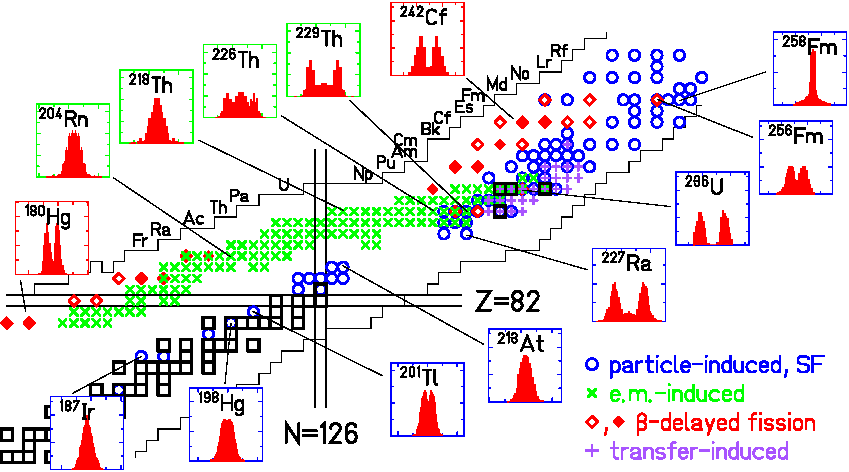
\includegraphics[width=0.9\linewidth]{./TeX_files/178Pt_region}
	\caption[Survey of fragment yields near $^{180}$Hg]{Fragment yields for several nuclei ranging from actinides, where primary fission yields tend to be asymmetric, down to near-thorium, where yields become more symmetric except in the region near neutron deficient {\Hg}. Figure from \cite{Andreyev2018}.}
	\label{fig:178ptregion}
\end{figure}



\section{Multimode fission of $^{178}$Pt}

One particular follow-up experiment was performed investigating spontaneous fission of {\Pt} \cite{our-Pt-paper}, which differs from {\Hg} by 2 protons. This system was studied at various excitation energies and found to fission consistently with a bimodal pattern, as shown in Figure \ref{fig:178ptexptdata}. Of the nuclei which underwent spontaneous fission, roughly 1/3 were found to fission symmetrically while the other 2/3 fissioned asymmetrically with a light-to-heavy mass ratio of approximately 79/99. Furthermore, it was observed that symmetric fragments tended to have higher kinetic energies than non-symmetric fragments.

\begin{figure}
	\centering
	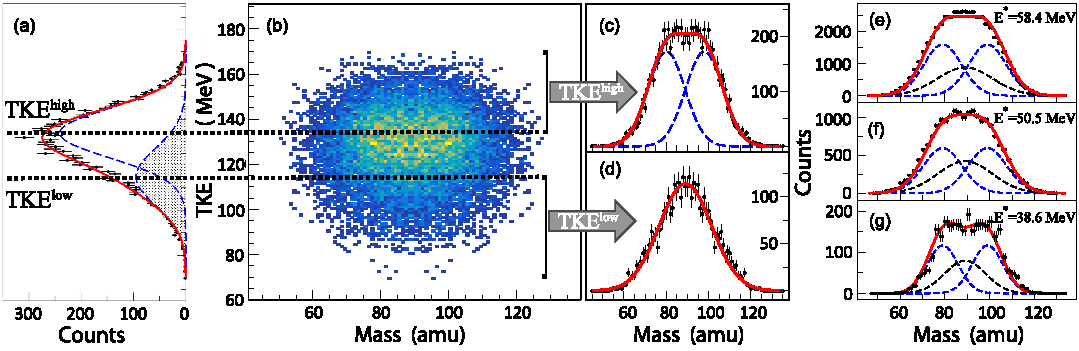
\includegraphics[width=0.95\linewidth]{TeX_files/178Pt_expt_data}
	\caption[$^{178}$Pt experimental data]{This figure contains the data from the {\Pt} experiment. I should go through and describe what all the individual boxes are for. Then I should cite out paper, once it's citeable}
	\label{fig:178ptexptdata}
\end{figure}

To better interpret the results of this experiment, DFT calculations were performed using the functionals {\hfb} \cite{Schunck2015} and D1S \cite{Berger1989}. These calculations involved computing a PES using the collective coordinates $Q_{20}$ and $Q_{30}$. [Do I need to describe the calculations in detail here, or should I refer to the published papers (e.g. ``Details of the calculation are given in \verb|the paper|'')?]

The {\hfb} PES is shown in Figure \ref{fig:178ptunedf1pes}, while the D1S PES is in Figure \ref{fig:178ptd1spes}. A calculation with full Langevin dynamics was not performed; however, the static (minimum-energy) pathway shown in the figure corresponds to a fragment split $A_L/A_H \approx 80/98$.

\begin{figure}
	\centering
	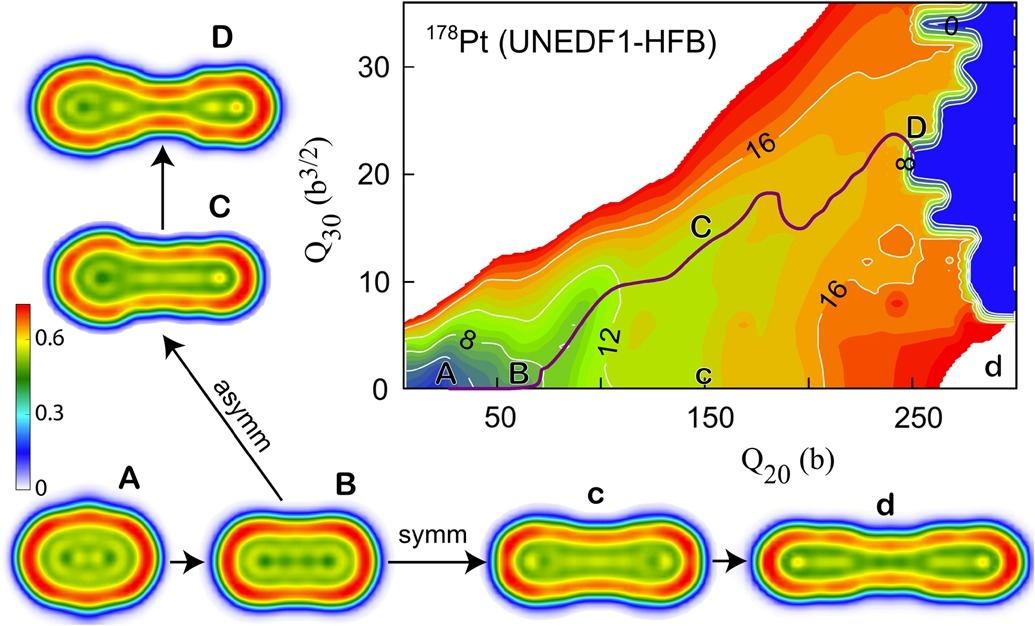
\includegraphics[width=0.7\linewidth]{TeX_files/178Pt_unedf1_pes.jpg}
	\caption[UNEDF1-HFB potential energy surface for $^{178}$Pt]{UNEDF1-HFB potential energy surface for $^{178}$Pt. Note the two different trajectories ABCD and ABcd and their corresponding localizations.}
	\label{fig:178ptunedf1pes}
\end{figure}

Also shown in Figure \ref{fig:178ptunedf1pes} are nucleon localization functions (recall Section ) corresponding to various configurations in the PES. Along the symmetric path (ABcd in the figure), the fragments appear highly-elongated, with a rather large neck, even shortly before scission. Since elongation tends to minimize the Coulomb repulsion between fragments, then this configuration might be expected to lead to fragments with relatively low kinetic energies. On the other hand, compact fragments such as those in ABCD will tend to have a larger Coulomb repulsion, propelling the fragments away from one another with greater force and resulting in fragments with a higher kinetic energy. [We note that this is compatible with experiment]

Now consider the PES corresponding to the D1S functional in Figure \ref{fig:178ptd1spes}. We note with some relief that, despite the inherent differences between the functionals, and despite the relative flatness of the surface with few discernible topological features, the overall topology of the PES is similar in both cases. The overall magnitude is different, but the static pathway follows a similar trajectory.

\begin{figure}
	\centering
	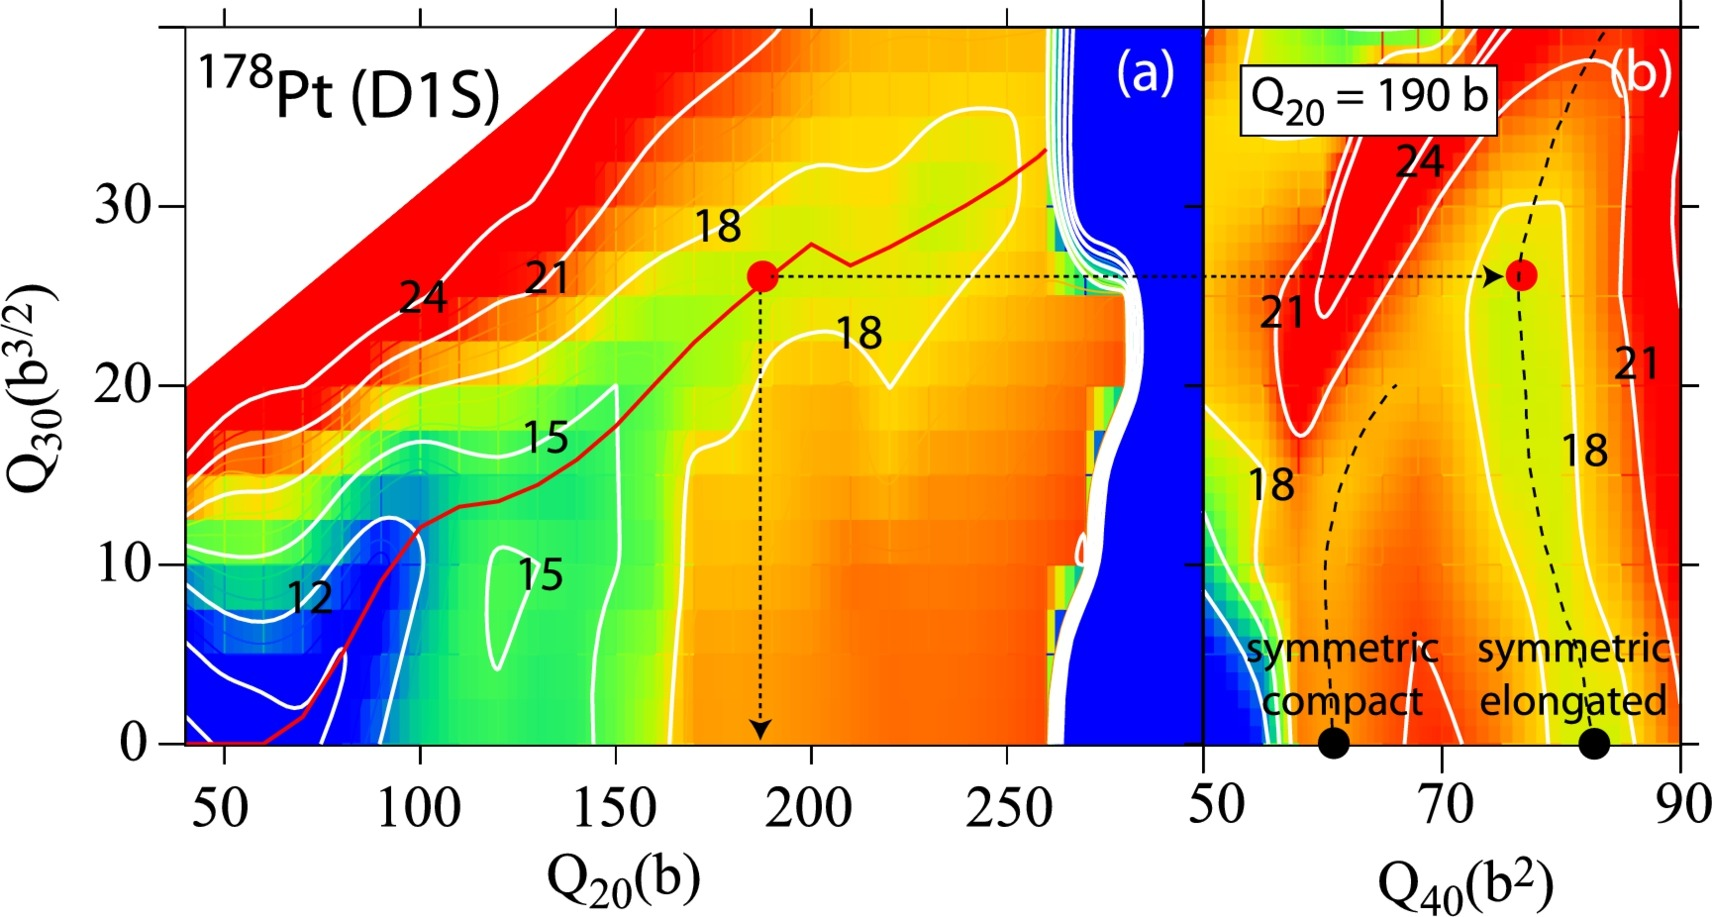
\includegraphics[width=0.7\linewidth]{TeX_files/178Pt_D1S_pes.jpg}
	\caption[D1S potential energy surface for $^{178}$Pt]{D1S potential energy surface for $^{178}$Pt. Note also the additional information about the hexadecapole moment.}
	\label{fig:178ptd1spes}
\end{figure}



\section{The physical origin of fragment asymmetry in the region of $^{180}$Hg}

Why is there a region of symmetric fission below thorium?

(These are notes from the 178Pt paper draft. Not mine, of course, but they have some good points to address): ``Namely, the PES are predicetd to be flat and much less structureless, and defined predominantly by the large liquid drop/macroscopic contribution, rather than by relatively small microscopic effects. Due to this, FFMDs exhibit fairly low dependence..  [refer to 180Hg PLB, as one example].

``(this was an answer by Witek, when somebody asked a question to my talk at Tsukuba - why the lead region is less sensitive to temperature.. the answer was - there is no 'barrier' in a sence, it's just flat/thick macroscopic surface, hardly influenced by shell effects.. so, even if one heats it up, tiny shell effects will be gone, but the main underlying macroscopic part will remain).''

Peter Moller argues in the concluding discussion of (https://link.aps.org/doi/10.1103/PhysRevC.85.024306 \cite{Moller2012}) that we can't really use the fragment/prefragment shell structure arguments in this region, and thus that we have yet to identify all the essential physics which determines fragments. He says the yields are given (at least in this case) by subtle interplays in local regions of the potential energy surface.

Witek, Michal Warda, and Staszczak argue in Section IV. \textit{Prescission Configurations} of \cite{Warda2012a} that 180Hg deforms as a molecular system consisting of 90Zr and 72Ge, with the remaining neck nucleons being distributed at scission to give the fragments they found in the experiment. Similarly, they make the same claim for 198Hg, except using 98Zr and 80Ge. The first one kind of makes sense to me since 90Zr is semi-magic, but 98Zr is not and neither is 80Ge. I wonder what might have happened had they tried to match up the densities of a different set of nearby nuclei (they used these because they had the same N/Z ratio as the fissioning parent nucleus). Then in the conclusions: ``We conclude that the mass distribution of fission fragments in both nuclei is governed by shell structure of prescission configurations associated with molecular structures.''

In the introduction to \cite{Mcdonnell2014} it is stated as though conclusively that ``the main factor determining the mass split in fission are shell effects at pre-scission configurations, i.e., between saddle and scission'' (see also some additional references therein). I think the thing that is most selling it to me so far, though, is Fig. 3 from this paper, wherein they show the shell correction energy for each of the nuclei considered. Even though the PES itself is mostly flat in each of these cases, the magnitude of the shell correction is different whether you are looking at symmetric or asymmetric trajectories, and the one with the larger magnitude shell correction happens to be the one that wins out in the final fragment distribution. I'd also be curious to see what the collective inertia looks like, but this seems to at least give something. It's not like this shell correction gets added on top of the PES - the PES is still relatively-flat - but it at least gives an explanation for why our traditional physical intuition is not totally failing us here.

Interesting future work in this region might include calculations with full dynamics (including from nuclei with excitation energy), as suggested in the conclusions of \cite{Mcdonnell2014}






